%%%%%%%%%%%%%%%%%%%%%%%%%%%%%%%%%%%%%%%%%%%%%%%%%%%%%%%%%%%%%%%%%%%%%%%%
%                                                                      %
%     File: Thesis_Implementation.tex                                  %
%     Tex Master: Thesis.tex                                           %
%                                                                      %
%     Author: Francisco Mendes                                         %
%     Last modified :  28 Nov 2019                                     %
%                                                                      %
%%%%%%%%%%%%%%%%%%%%%%%%%%%%%%%%%%%%%%%%%%%%%%%%%%%%%%%%%%%%%%%%%%%%%%%%

\chapter{Proposal}
\label{chapter:implementation}


\begin{figure}[!htb]
  \centering
  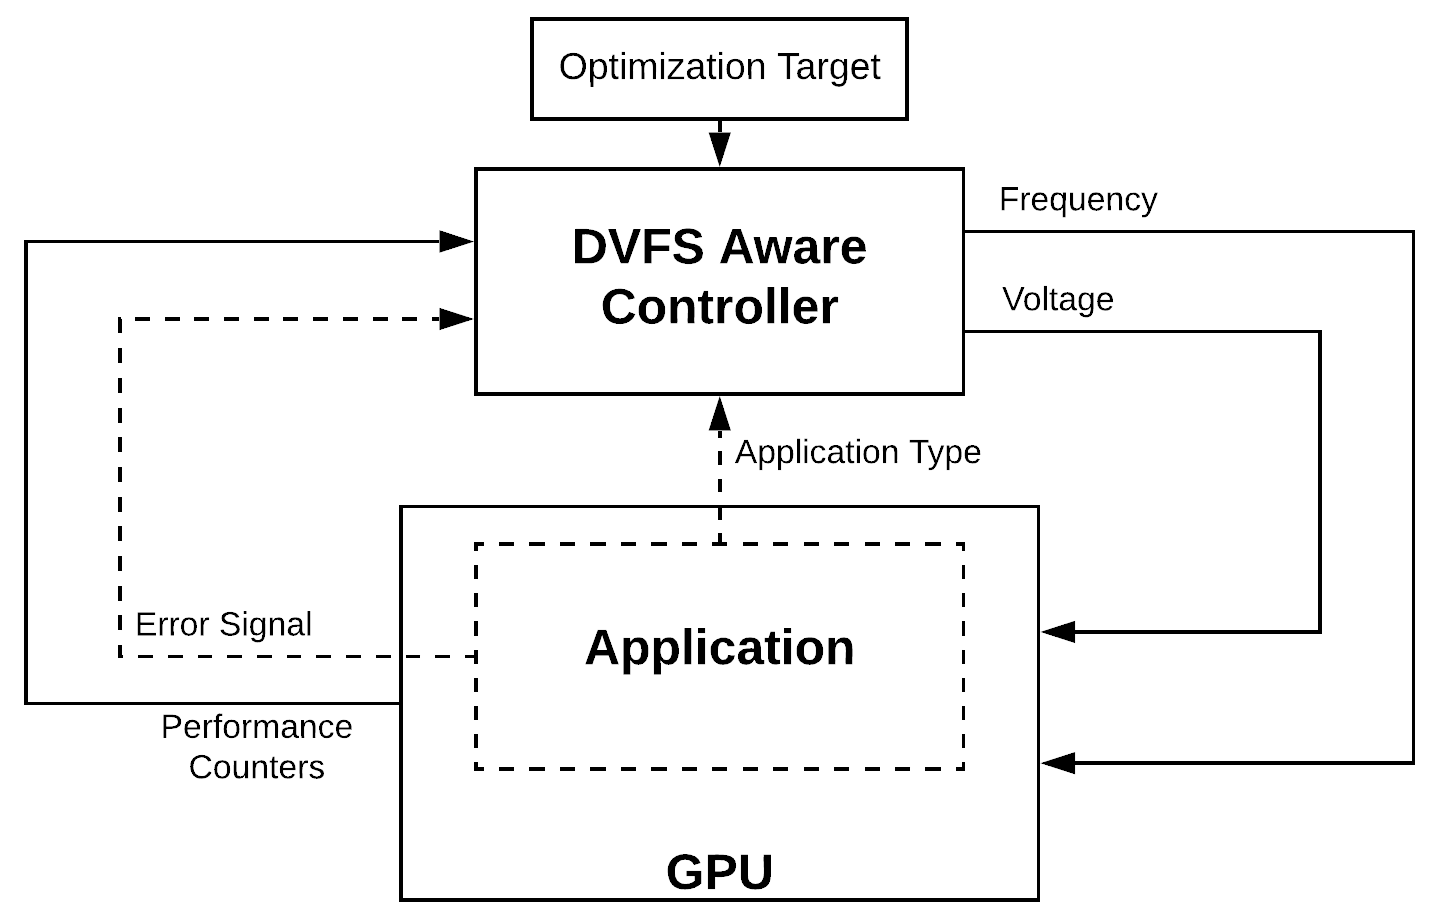
\includegraphics[width=0.75\textwidth]{Figures/Proposel/DVFS_Aware_Controller.png}
  \caption[Controller]{DVFS Aware Controller Block Diagram.}
  \label{fig:controlerDVFSaware}
\end{figure}


\section{Experimental Methodology}

To design the controller, it is necessary to first identify a set of artificial neural network models that are imprecision tolerant. Then, acquire meaningful metrics about the state of the GPU core and the quality of the output that the neural networks are producing. The second step is to study the relation between 

Analisar o comportamento da arquitetura da GPU à mudança de DVFS

Entender o comportamento da aprendisagem de modelos de machine learning - redes neuronais em particular - aquando da variação do ponto de funcionamento da GPU

Arranjar uma metodologia de analise da qualidade do output da aplicação e do estado do GPU

De modo a desenhar um controlador de tensao e frequencia realimentado 

\section{GPU non-convectional DVFS characterization}
\subsection{Fundamental Analysis}

\subsection{DNN Primitives Analysis}

%%%%%%%%%%%%%%%%%%%%%%%%%%%%%%%%%%%%%%%%%%%%%%%%%%%%%%%%%%%%%%%%%%%%%%%%
\section{GPU DVFS Aware Mechanism}
\label{section:DVFSaware}

%DVFS-aware application classification to improve GPGPUs energy effciency
Utilizar estrategia daqui como inicio -> treinar ANN
%%%%%%%%%%%%%%%%%%%%%%%%%%%%%%%%%%%%%%%%%%%%%%%%%%%%%%%%%%%%%%%%%%%%%%%%
\subsection{Architecture of the Solution}
\label{section:solarch}


\subsection{DNN Models Optimization}